% !TEX root = ../my-thesis.tex
%

\chapter{Analysis of Geospatial Health Data}
\label{sec:geodata}
Healthcare data provides information for detecting public health problems and reacting adequately when they occur. With this information, prevention and control of a multitude of health conditions including infectious diseases, non-communicable diseases, injuries and health-related behaviours can be achieved. To analyse and interpret health data, the process involves a wide variety of system designs, analytical methods, modes of presentation and interpretive uses\autocite[][]{teutsch2000principles}. Descriptive methods generally form the basis of routine reporting of surveillance data. Rather than focusing on observed patterns in the data, these may also attempt to compare the relative occurrence of health outcomes in different subgroups. More specific hypotheses can be explored using inferential methods. The aim of these methods is to draw statistical inferences about patterns or outcomes of health. \\
The increasing availability of geo-referenced health data, population data, satellite imagery of environmental factors influencing levels of disease activity, and the development of geographic information systems (GIS) and address geocoding software, the rise of studies of spatial and spatio-temporal variation in disease has been facilitated. John Snow's investigation of the cholera outbreak in London in 1854 offers one of the most well-known examples of spatial analysis. By using a map, Snow illustrated how cholera deaths seemed to accumulate around a public water pump. Evaluating the spatial pattern of cholera cases was essential to identify the source of infection and supported the theory of cholera transmission through drinking water \autocite[][]{snow1857cholera}. \\
A broad range of spatial and spatio-temporal methods exist for disease surveillance, including methods for disease mapping, clustering and geographic correlation studies. These methods can be used to identify areas of high risk, risk factors, evaluate spatial variations in temporal trends, measure excess disease risk near a suspected source and detect outbreaks at an early stage.
\clearpage
\section{Geographic Data}
In spatial statistics, two fundamental types of geographic data exist, namely \textit{vector data} and \textit{raster data}. In the vector data model, the world is represented by points, lines and polygons with discrete, well-defined boundaries, which tends to result in high accuracy. Raster data, on the other hand, divides the surface into cells of uniform size, and raster datasets are used as the basis for background images in web mapping. \\
Determining which data type to use depends on the domain of the application. Vector data dominates in the social sciences because human settlements typically have discrete boundaries, while raster data are commonly used in many environmental sciences because they are based on remote sensing data. Naturally, there is also some overlap and both types can be used together or one form can be converted into the other \autocite[][]{lovelace2019geocomputation}.
\subsection{Vector Data}
The geographic vector data model is based on points located within a \textit{coordinate reference system} (CRS), in which points either represent self-standing features or form more complex geometric shapes, i.e. lines and polygons. Using this system, Trondheim can be represented by the coordinates $\left(10.4, 63.4\right)$, meaning $10.4$ degrees east of the prime meridian and $63.4$ degrees north of the equator. It could also be written as $\left(1157722.70, 9199010.75\right)$, which is the position of Trondheim using the Web Mercator projection, the de facto standard for web mapping applications. More will be said about CRS later, but for now it is sufficient to know that it is possible to display coordinates in various ways. An example of a CRS is shown in Figure~\ref{fig:globe}.
\begin{figure}[H]
   \centering
       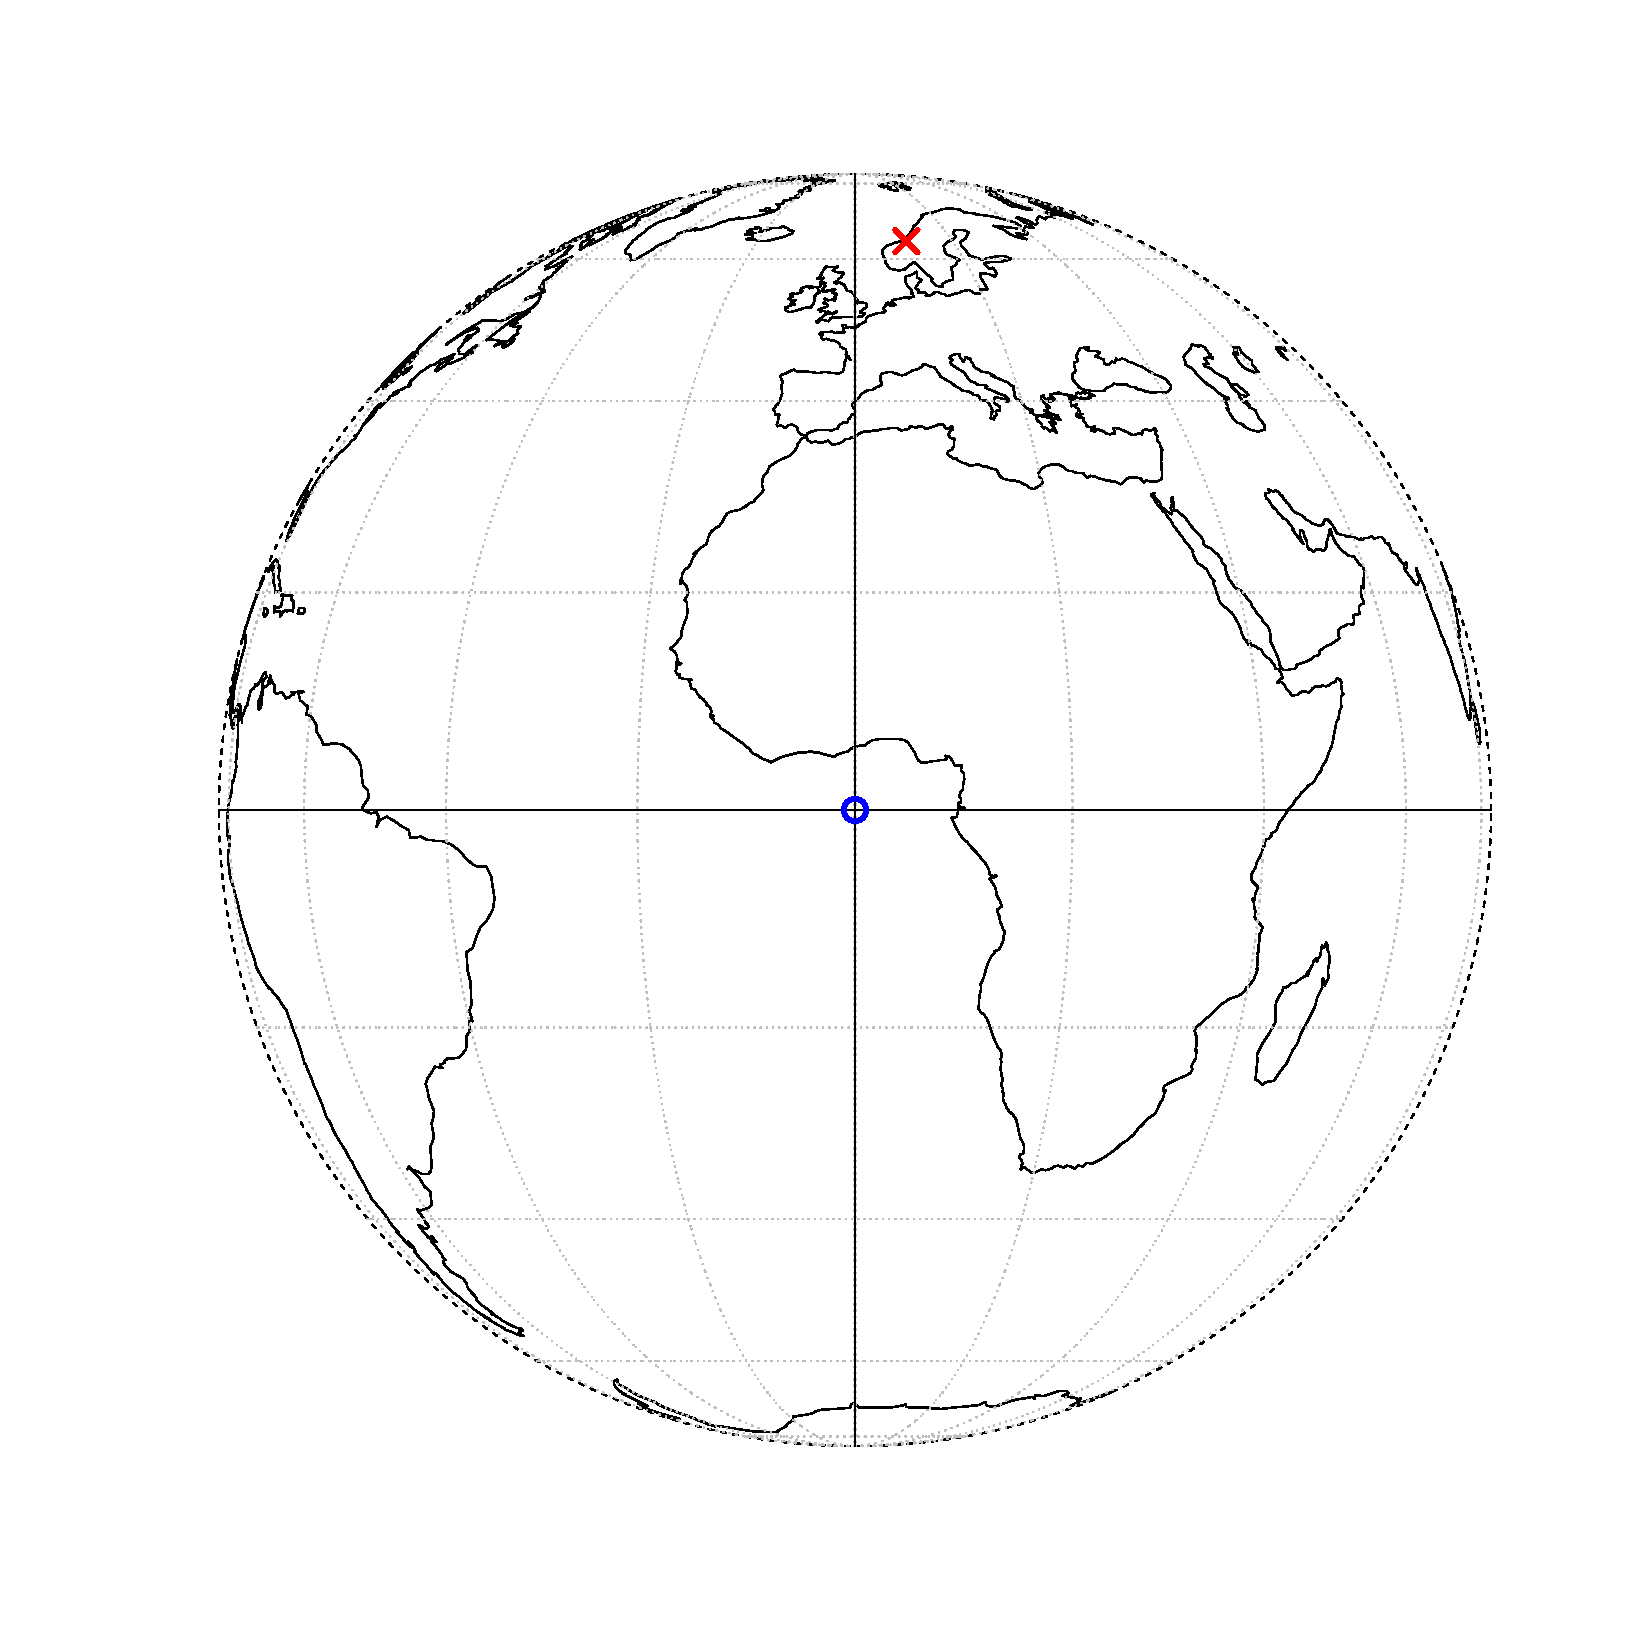
\includegraphics[page=1,width=.7\textwidth]{globe.pdf}
 \caption{A geographic CRS with an origin at 0° longitude and latitude. The red X denotes the location of Trondheim.}
 \label{fig:globe}
\end{figure}
\subsubsection*{Different Types of Vector Data}
As mentioned earlier, there are different types of vector data. There are 17 different geometry types in the standard \textit{simple features}, but there are seven core types that can be used in most analysis software. These types are visualised in Figure~\ref{fig:sf}.
\begin{figure}[H]
   \centering
       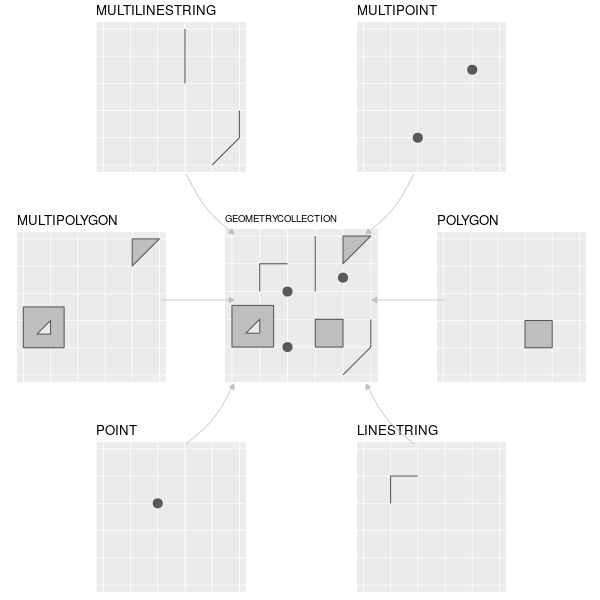
\includegraphics[width=.7\textwidth]{sf-classes.png}
 \caption{The most commonly used simple feature types.}
 \label{fig:sf}
\end{figure} $\newline$
Simple Features was developed by the Open Geospatial Consortium and is an open, standardised, hierarchical data model that represents a wide range of geometry types. The use of this data model ensures that scientific work can be transferred to other institutions, e.g. when importing from and exporting to spatial databases \autocite[][]{lovelace2019geocomputation}. 
\subsection{Raster Data}
The geographic raster data model consists in most cases of a raster header and a matrix representing uniformly distributed cells/pixels. The raster header defines the CRS, the origin (starting point) and the extent. Since the number of columns and rows and the resolution of the cell size are stored in the extent, starting from the origin, it is easy to access and change each cell by its ID or by specifying the row and column number. In this type of representation, the coordinates of the four vertices of each cell are not explicitly stored, instead only the origin is stored. This speeds up data processing and makes it more efficient, but each raster layer can only contain a single value, which can be either numeric or categorical. Typically, raster maps are used to depict continuous features such as elevation or temperature, but categorical variables, for example soil or land cover, as shown in Figure~\ref{fig:raster} \autocite[][]{lovelace2019geocomputation}.
\begin{figure}[H]
   \centering
       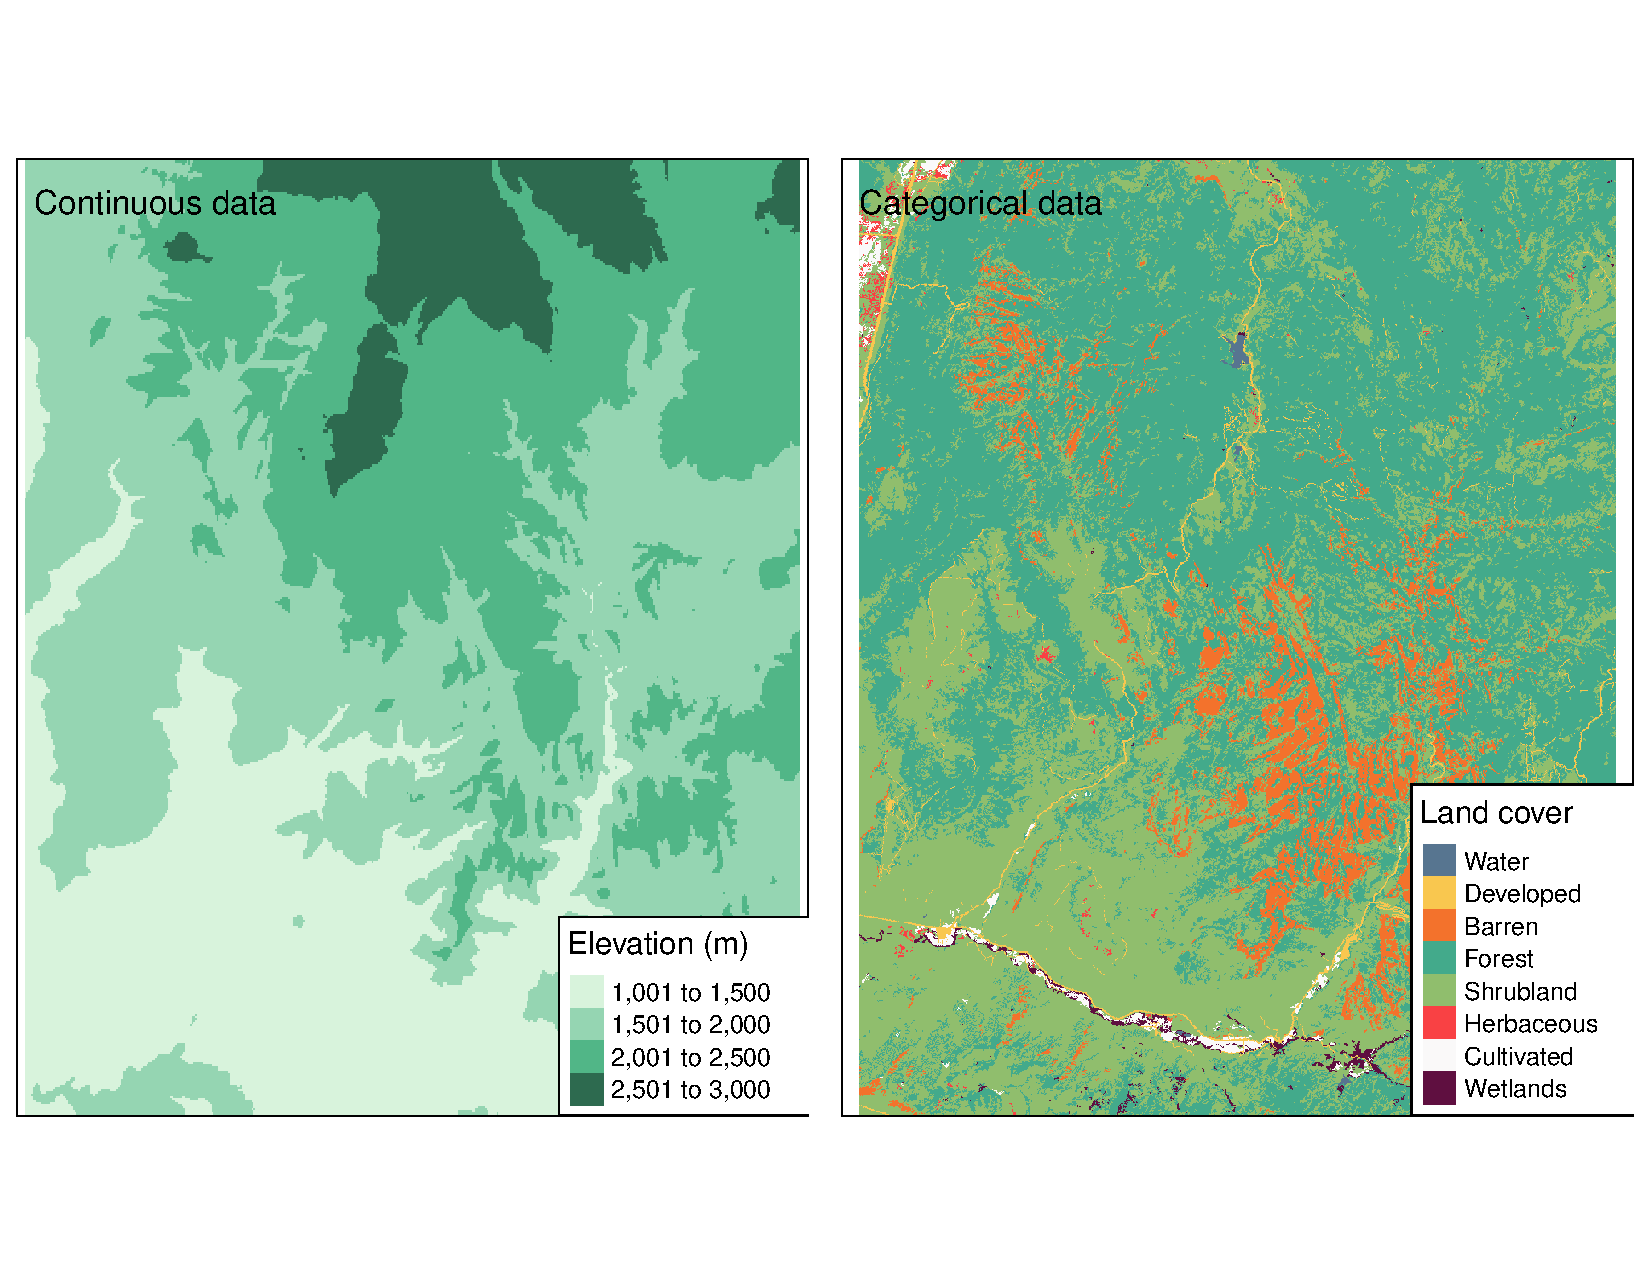
\includegraphics[page=1,width=\textwidth]{raster.pdf}
 \caption{An example of continuous and categorical raster data}
 \label{fig:raster}
\end{figure}
\subsection*{Coordinate Reference Systems}
A common denominator of vector and raster data are that both use the coordinate reference system (CRS), which defines how spatial elements relate to the surface of the Earth. The CRS can be either geographic or projected.
\subsubsection*{Geographic Coordinate Systems}
Geographic coordinate systems use two values, \textit{longitude} and \textit{latitude}, to identify any location on Earth. Longitude is defined as the east-west location at an angular distance from the prime meridian plane, while latitude is the angular distance north or south of the equator. Consequently, distances in geographic CRS are not measured in metres. \\
The Earth's surface is typically represented in geographical coordinate systems by a spherical or ellipsoidal surface. The former assumes that the Earth is a perfect sphere of a certain radius, which has the advantage of being a simplistic model, but is associated with inaccuracies owing to the fact that the Earth is not a sphere. Ellipsoidal models are defined by the equatorial radius and the polar radius, providing a better model since the equatorial radius is approximately 11.5 km longer than the polar radius.\\
The \textit{datum} is a broader component of CRS that contains information about which ellipsoid to use and the exact relationship between Cartesian coordinates and the location on the Earth's surface. The notation \textit{proj4string} is used to store these additional details. It allows for local variations of the Earth's surface, such as large mountain ranges, to be taken into account in local CRS. Datum can again be divided into two categories, \textit{local} and \textit{geocentric}, the difference being that in the local datum the ellipsoidal surface is shifted to match the surface at a particular location, whereas in the geocentric datum the centre of gravity of the Earth is the centre and the accuracy of the projections is not optimised for any particular location \autocite[][]{lovelace2019geocomputation}.
\subsubsection*{Projected Coordinate Systems}
Projected CRS are based on Cartesian coordinates on an implicitly flat surface and have an origin, $x$ and $y$ axes, and a linear unit of measurement, metres for instance. They are based on geographic CRS and rely on map projections to convert between the three-dimensional surface of the Earth and the east/north values ($x$ and $y$) in a projected CRS.\\
This transition always entails some distortion, skewing some of the properties of the earth's surface, such as area, direction, distance and shape. Generally, the name of a projection is based on a property it preserves, e.g. equal area projection preserves area, equidistant projection preserves distance and conformal projection preserves local shape. \\
Again, subgroups exist in projection coordinate systems, \textit{conic}, \textit{cylindrical} and \textit{planar} projections. In a conic projection, the earth's surface is projected onto a cone along one or two tangent lines. Along these lines the distortions are minimised and increase with the distance to the lines. The projection is therefore best suited for maps of mid-latitude areas. Cylindrical projections map the surface onto a cylinder. These types of projections can be created by touching the surface of the Earth along one or two tangent lines. They are often used to map the entire Earth. A planar projection projects data onto a flat surface that touches the globe at a point or along a tangent line, and is typically used in mapping polar projections \autocite[][]{lovelace2019geocomputation}.
\clearpage
\section{Spatial Point Processes}
A stochastic process that describes the location of particular events/points that occur in a region is known as a point process. The number of points as well as the location of the points are random. An example of a point process would be the number of earthquakes and their locations.
\subsection{Fundamentals of Point Processes}
Let $Z$ be a random, at most countable set of points in a space $\mathbb{X}$, for example $\mathbb{R}^d$. Ignoring measurability issues, $Z$ can be thought of as a mapping $\omega\mapsto Z\left(\omega\right)$ from $\Omega$ into the set of countable subsets of $\mathbb{X}$, where $\left(\Omega, \mathcal{F}, \mathbb{P}\right)$ defines an underlying probability space. $Z$ can then be identified with the family of mappings
\begin{equation}
    \omega\mapsto\eta\left(\omega, B\right):=\hbox{card}\left(z(\omega)\cap B\right), \hspace{20pt}B\subset\mathbb{X},
\end{equation}
which counts the number of points from $Z$ in $B$. For any fixed $\omega\in\Omega$, $\eta\left(\omega,\cdot\right)$ is the counting measure supported by $Z\left(\omega\right)$ \autocite[][]{cox1980point}. \\
For a general definition of a point process, let $\left(\mathbb{X}, \mathcal{X}\right)$ be a measurable space and let $N_{<\infty}\left(\mathbb{X}\right)\equiv N_{<\infty}$ be the space of all measures $\mu$ on $\mathbb{X}$ such that $\mu(B)\in\mathbb{N}_0: =\mathbb{N}\cup\lbrace0\rbrace\,\forall B\in\mathcal{X}$. Let $N\left(\mathbb{X}\right)\equiv N$ be the space of all measures describable as a countable sum of measures from $N_{<\infty}$, for example the \textit{zero measure} 0 which is equal to $0$ on $\mathcal{X}$. In general, any sequence $\left(x_n\right)_{n=1}^k$ of elements of $\mathbb{X}$, where $k\in\overline{\mathbb{N}}:=\mathbb{N}\cup\lbrace\infty\rbrace$ denotes the number of terms in the sequence, can be used to define a measure
\begin{align}
    \mu&=\sum_{n=1}^k\delta_{x_n}. \label{eq:measure} \\
    \Rightarrow\mu\left(B\right)&=\sum_{n=1}^k\pmb{1}_B\left(x_n\right),\hspace{20pt} B\in\mathcal{X}. \nonumber
\end{align}
More generally, for any measurable $f:\mathbb{X}\rightarrow\left[0,\infty\right]$,
\begin{equation}
    \int fd\mu=\sum_{n=1}^kf\left(x_n\right)
\end{equation}
For $k=0$ in \eqref{eq:measure}, $\mu$ is equal to the zero measure. The point set $\pmb{x}=\left(x_1,...,x_n\right)^T$ is said to be not pairwise different and if $x_i=x_j$ with $i\neq j$, $\mu$ is said to have multiplicities. The multiplicity of $x_i$ is equal to the number
\begin{equation*}
    \hbox{card}\left\lbrace j\leq k:x_j=x_i\right\rbrace.
\end{equation*}
Any $\mu$ of the form \eqref{eq:measure} is interpreted as a counting measure with possible multiplicities, but in general it cannot be guaranteed that every $\mu\in N$ can be written in this particular form. \\
A point process $\eta$ on $\mathbb{X}$ is called \textit{proper point process} if random elements $X_1,X_2,...\hbox{exist} \in \mathbb{X}$ and a $\overline{\mathbb{N}}_0$-valued random variable $\kappa$ such that almost surely
\begin{equation}
    \eta=\sum_{n=1}^{\kappa}\delta_{X_n}.
\end{equation}
For $\kappa=0$ this is the zero measure on $\mathbb{X}$. \\
This terminology is motivated by the intuition that a point process is a (random) set of points, rather than an integer measure. A proper point process fits this intuition better, since it can be interpreted as a countable set of points in $\mathbb{X}$ \autocite[][9--12]{last2017lectures}.
\subsection{Poisson Processes}
Poisson processes are defined by the fact that the number of points in a given set follows a Poisson distribution. Furthermore, the numbers of points in disjoint sets are stochastically independent. \\
In application, Poisson processes are used in a wide range of fields, including biology, economics and image processing. \\
Let $\lambda$ be an $s$-finite measure on $\mathbb{X}$. Let a \textit{Poisson process} with intensity measure $\lambda$ be defined as a point process $\eta$ on $\mathbb{X}$ with the following two properties:
\begin{itemize}
    \item[1.] $\forall B\in\mathcal{X}: \eta\left(B\right)\sim\hbox{Po}\left(\lambda(B);k\right)\forall k\in\mathbb{N}_0 \Longleftrightarrow \mathbb{P}\left(\eta\left(B\right)=k\right)$
    \item[2.] 
    $\forall m\in\mathbb{N}$ and all pairwise disjoint sets $B_1,...,B_m\in\mathcal{X}:$ the random variables $\eta\left(B_1\right),...,\eta\left(B_m\right)$ are independent.
\end{itemize}
A point process satisfying the second of these conditions is called \textit{completely independent}. If $\eta$ is a Poisson process with intensity measure $\lambda$, then
\begin{equation}
    \mathbb{E}\left[\eta\left(B\right)\right]=\lambda(B).
\end{equation}
For the zero measure,
\begin{equation*}
    \mathbb{P}\left(\eta(\mathbb{X})=0\right)=1,
\end{equation*}
with $\lambda=0$ \autocite[][19]{last2017lectures}.

% \subsection{Random Measures and Cox Processes}
% A Poisson process with a random intensity measure, and thus the result of a \textit{doubly stochastic} process, is called a \textit{Cox process}. A random measure is a natural and important generalisation of a point process and it is the determining factor of the distribution of a Cox process. \\
% Since a Cox process $\eta$ can be interpreted as the result of a doubly stochastic process, a random measure $\xi$ is generated first, followed by a Poisson process with intensity measure $\xi$. \\
% These processes are often used to simulate spike trains or in financial mathematics for modeling the prices of financial instruments where credit risk is a major factor.
% \subsubsection{Random Measures}
% Let $\left(\mathbb{X}, \mathcal{X}\right)$ be a measurable space and let $M\left(\mathbb{X}\right)\equiv M$ denote the set of all $s$-finite measures $\mu$ on $\mathbb{X}$. Let $\mathcal{M}\left(\mathbb{X}\right)\equiv \mathcal{M}$ be the $\sigma$ field generated by all sets of the form
% \begin{equation*}
%    \left\lbrace\mu\in M:\mu(B)\leq t\right\rbrace, \hspace{20pt}B\in\mathcal{X}, t\in\mathbb{R}_{+}.
% \end{equation*}
% This is equal to the smallest $\sigma$-field of subsets of $M$ such that $\mu\mapsto\mu(B)$ is a measurable mapping for all $B\in\mathbb{X}$. \\
% A random measure on $\mathbb{X}$ is defined as a random element $\xi$ of the space $\left(M,\mathcal{M}\right)$, i.e. a measurable mapping $\xi:\Omega\mapsto M$. \\
% If $\xi$ is a random measure and $B\in\mathcal{X}$, then $\xi(B)$ denotes the random variable $\omega\mapsto\xi\left(\omega,B\right):=\xi\left(\omega\right)(B)$. This mapping represents a kernel from $\Omega$ to $\mathbb{X}$ with the additional property that the measure $\xi\left(\omega,\cdot\right)$ is $s$-finite for each $\omega\in\Omega$. \\
% A random measure $\xi$ on $\mathbb{X}$ follows the distribution of the probability measure $\mathbb{P}_{\xi}$ on $\left(M,\mathcal{M}\right)$ given by $A\mapsto\mathbb{P}\left(\xi\in A\right)$. This distribution is again determined by the family of random vectors $\left(\xi\left(B_1\right),...,\xi\left(B_m\right)\right)$ for pairwise disjoint $B_1,...,B_m\in\mathcal{X}$ and $m\in\mathbb{N}$  \autocite[][127--128]{last2017lectures}.
% \subsubsection{Cox Processes}
% Let $\Pi_{\lambda}$ denote the distribution of a Poisson process with intensity measure $\lambda\ in M\left(\mathbb{X}\right)$ and let $\xi$ be a random measure on $\mathbb{X}$. A point process $\eta$ on $\mathbb{X}$ is called a Cox process directed by $\xi$ if
% \begin{equation}
%    \mathbb{P}\left(\eta\in A|\xi\right)=\Pi_{\xi}(A),\hspace{20pt}\mathbb{P}\hbox{-almost surely}, A\in\mathcal{N}.
% \end{equation}
% $\mathcal{N}\left(\mathbb{X}\right)\equiv\mathcal{N}$ denotes the $\sigma$ field formed by the set of all subsets of $N$ of the form
% \begin{equation*}
%    \left\lbrace\mu\in N:\mu(B)=k\right\rbrace, \hspace{20pt}B\in\mathcal{X},k\in\mathbb{N}_0.
% \end{equation*}
% Thus $\mathcal{N}$ denotes the smallest $\sigma$ field on $N$ such that $\mu\mapsto\mu(B)$ is % measurable for all $B\in\mathcal{X}$  \autocite[][129]{last2017lectures}.
\clearpage
\section{Modeling and Visualising Health Data}
\subsection{Areal Data}
Areal or lattice data are the result of segmenting a fixed domain into a finite number of sub-regions where results are aggregated, e.g. the number of infections with a specific disease in districts or the number of overweight people in provinces. Often the aim of disease risk models is to assess the risk within the same areas for which data are available. This can be done with a simple measure such as the \textit{standardised incidence ratio} (SIR) or by using a Bayesian hierarchical model, which allows information to be drawn from neighbouring areas and incorporates covariates, thereby smoothing and reducing extreme values. \\
A widely used model is the \textit{Besag-York-Mollié} (BYM) \autocite[][]{besag1991bayesian}, which takes spatial correlation and the potential for observations in neighbouring areas to be more similar than those in distant regions into account. It includes a spatial random effect that smoothes the data according to a neighbourhood structure, and an unstructured exchangeable component that models uncorrelated noise. In settings where disease numbers are monitored over time, spatio-temporal models account for temporal correlations in addition to spatial correlation, while also accounting for spatio-temporal interactions  \autocite[][]{moraga2019geospatial}.
\subsubsection{Spatial Neighbourhood Matrices}
Spatial or proximity matrices are useful for exploratory analysis of area data. Let $w_{ij}$ denote the $\left(i,j\right)$ element of a \textit{spatial neighbourhood matrix} $\pmb{W}$. $w_{ij}$ connects the two areas in some spatial way. The neighbourhood structure over the complete study region is defined by $\pmb{W}$, and the elements of the matrix can be considered as weights. The closer $j$ is to $i$, the more weight is associated with it. The simplest neighbourhood definition is given by the binary matrix
\begin{equation}
    w_{ij}=\begin{cases}
    1 & \hbox{ if regions } i $\hbox{ and }$ j \hbox{ share a border} \\
    0 & \hbox{ else }
    \end{cases}
\end{equation}
Since a region cannot share a boundary with itself, $w_{ii}=0$  \autocite[][]{moraga2019geospatial}.\\
In Figure~\ref{fig:neighbour}, the number of shared borders of each canton in Switzerland are mapped.
\begin{figure}[H]
   \centering
       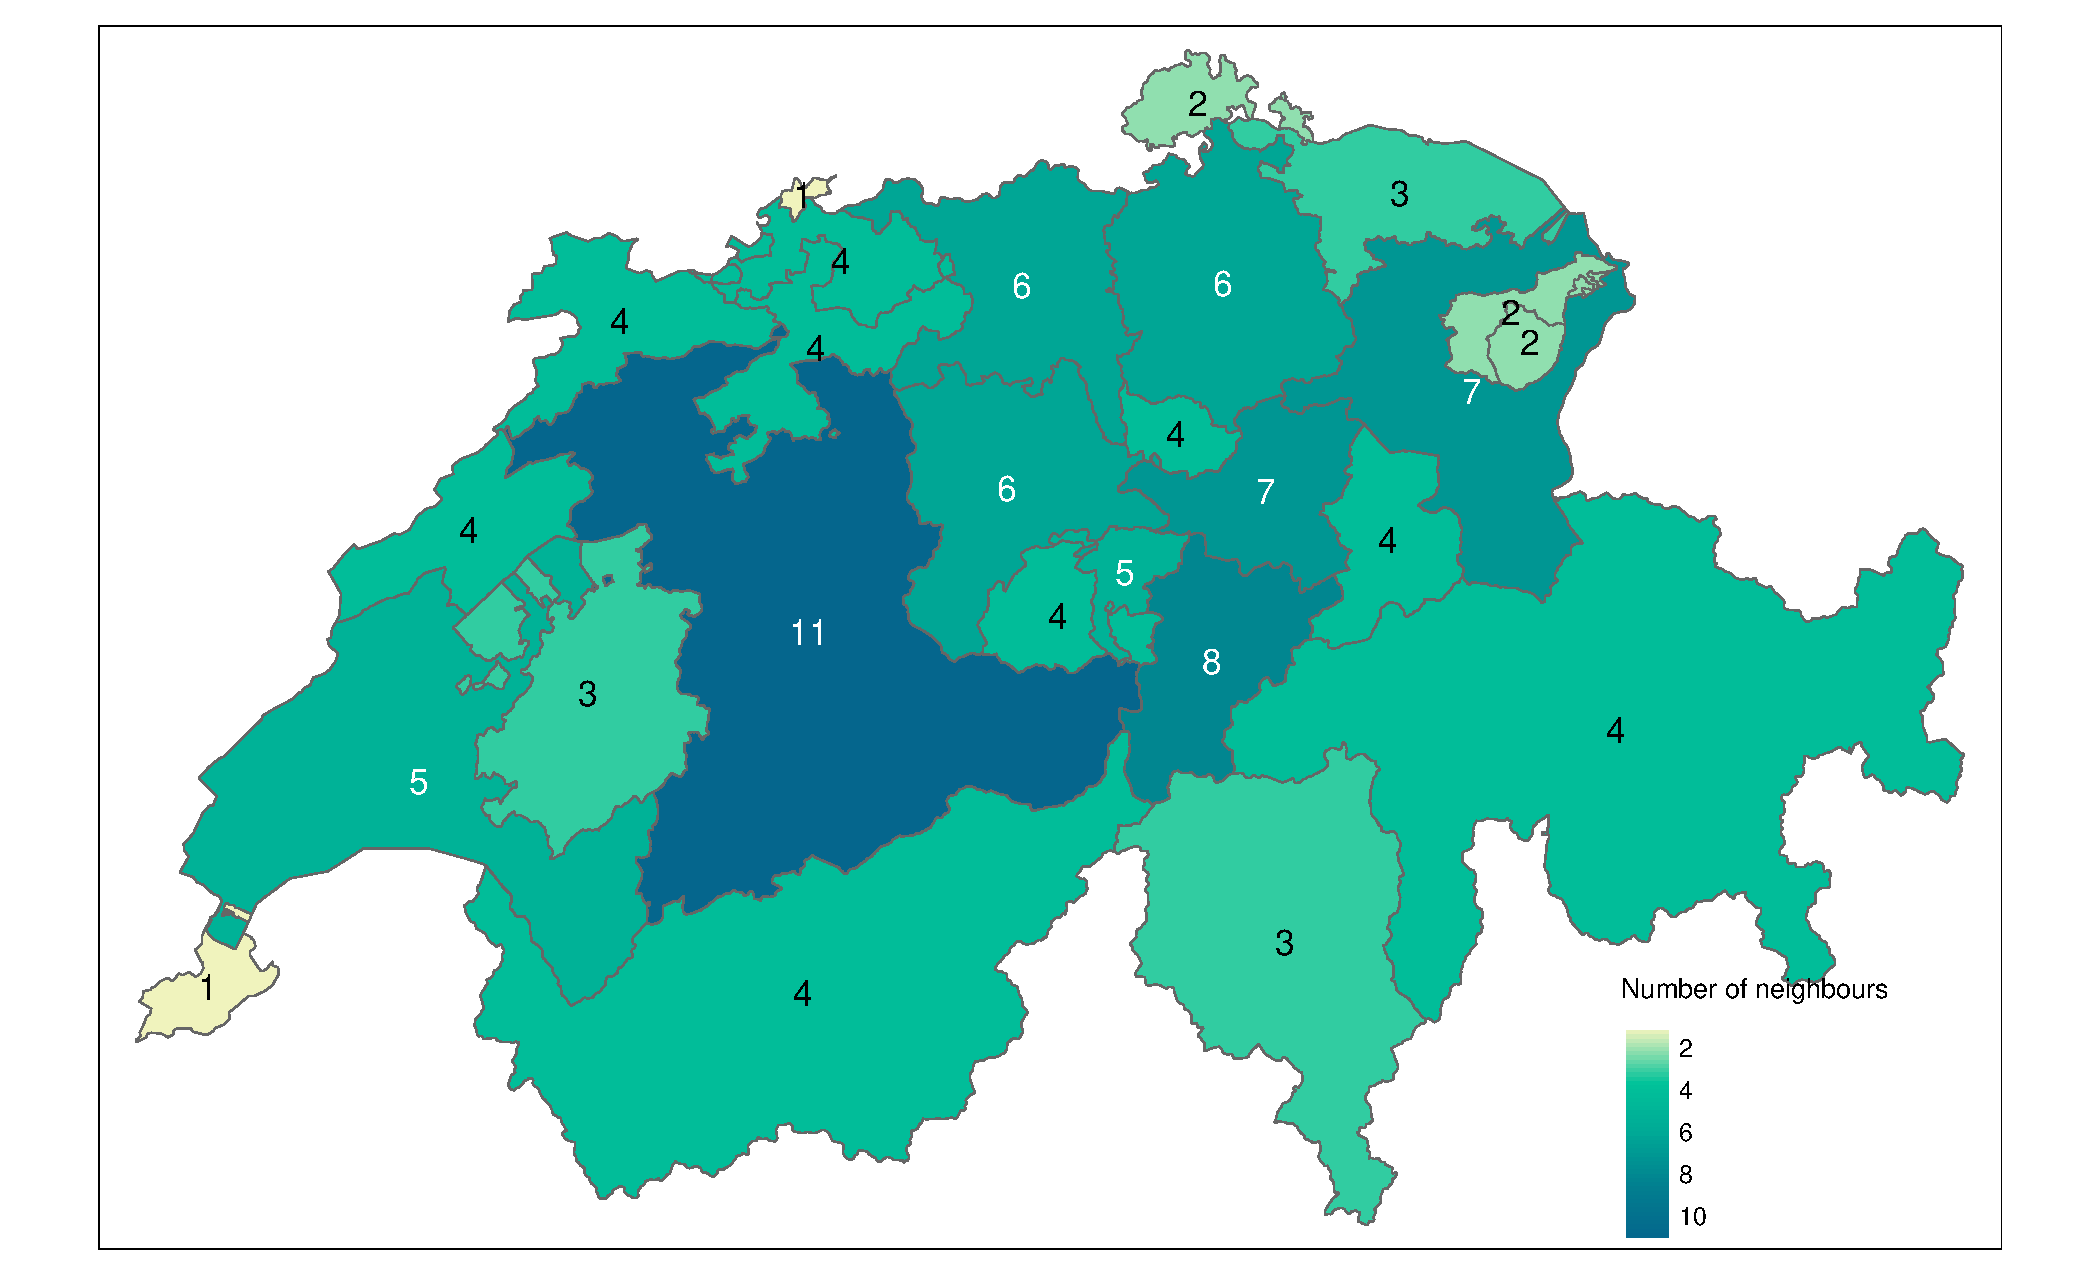
\includegraphics[page=1,width=\textwidth]{neighbours.pdf}
 \caption{The number of shared borders of cantons in Switzerland}
 \label{fig:neighbour}
\end{figure}
\subsubsection{Standardised Incidence Ratio}
A basic measure of disease risk is the \textit{standardised incidence ratio}, which yields an estimate in each of the areas that form a partition of the study region. It is defined as the ratio of observed counts to expected counts
\begin{equation}\label{eq:sir}
    \hbox{SIR}_i = \frac{Y_i}{E_i}.
\end{equation}
$E_i$ represents the sum of the expected number of cases of a given area $i$ that behave according to the way the standard population behaves. It is calculated using indirect standardisation as
\begin{equation}
    E_i=\sum_{j=1}^mr_j^{(s)}n_j^{(i)},
\end{equation}
with $r_j^{(s)}$ the rate in stratum $j$ in the standard population and $n_j^{(i)}$ the population in stratum $j$ of area $i$. If the stratum information is unavailable, the expected counts can be calculated as follows
\begin{equation*}
    E_i = r^{(s)}n^{(i)},
\end{equation*}
where $r^{(s)}$ denotes the rate in the standard population and $n^{(i)}$ is the population of area $i$. If the standardised incidence rate is greater than 1, area $i$ has a higher risk than expected from the standard population, while for $\hbox{SIR}_i = 1$ the risk is the same and for $\hbox{SIR}_i < 1$ it is lower than expected. The ratio is also called the standardised mortality ratio when applied to mortality data \autocite[][]{moraga2019geospatial}.
\subsubsection{Spatial Small Area Disease Risk Estimation}
While SIRs may prove useful in some situations, in areas with low population sizes or rare diseases, expected counts may be low, making SIRs insufficiently reliable for reporting. It is therefore preferable to assess disease risk using models that allow information to be borrowed from neighbouring areas and incorporate information from covariates, thus smoothing or shrinking extreme values due to small sample sizes \autocite[][]{gelfand2010handbook}. \\
The observed counts $Y_i$ in area $i$ are typically modeled with a Poisson distribution with mean $E_i\theta_i$, where $E_i$ is the expected counts and $\theta_i$ denotes the relative risk in area $i$. To account for extra Poisson reliability, the logarithm of the relative risk is expressed as the total of the intercept and the random effects. $\theta_i$ quantifies whether area $i$ has a higher $\left(\theta_i >1\right)$ or lower $\left(\theta_i <1\right)$ risk than the average risk in the standard population. If the risk of an area $i$ is half the average risk, then $\theta_i = 0.5$. The general model for spatial data is formulated as follows:
\begin{align}
    Y_i&\sim\hbox{Po}\left(E_i\theta_i\right), \hspace{20pt} i=1,...,n,\\
    \log\left(\theta_i\right)&=\alpha+u_i+v_i.
\end{align}
The overall risk in the region of study is represented by $\alpha$, $u_i$ is a random effect specific to each area to model the spatial dependence between relative risks, and $v_i$ is an unstructured exchangeable component that models uncorrelated noise, $v_i\sim\mathcal{N}\left(0,\sigma_v^2\right)$. Covariates are often included to measure risk factors and other random effects to deal with different sources of variability. For example,
\begin{equation*}
    \log\left(\theta_i\right)=\pmb{d}_i\pmb{\beta}+u_i+v_i,
\end{equation*}
with $\pmb{d}_i = \left(1,d_{i1},...,d_{ip}\right)$ a vector of the intercept and $p$ covariates corresponding to the area $i$ and $\pmb{\beta}=\left(\beta_0,...,\beta_p\right)^T$ the vector of coefficients. An increase in $d_j\,\left(j = 1,...,p\right)$ by one unit, leads to an increase in the relative risk by a factor of $\exp\left(\beta_j\right)$, provided that all other covariates remain constant. \\
In the Besag-York-Mollié (BYM) \autocite[][]{besag1991bayesian} model, this spatial random effect $u_i$ is assigned a conditional autoregressive (CAR) distribution that smooths the data according to a given neighbourhood structure that defines two areas as neighbours if they share a common boundary \autocite[][]{moraga2019geospatial}.
%Specifically,
% \begin{equation}
%     u_i|\pmb{u}_{-i}\sim\mathcal{N}\left(\overline{u}_{\delta_i}, \frac{\sigma_u^2}{n_{\delta_i}}\right),
% \end{equation}
% where $\overline{u}_{\delta_i}^{-1}=n_{\delta_i}^{-1}\sum_{j\in\delta_i} u_j$, while $\delta_i$ and $n_{\delta_i}$ represent the set and the amount of neighbours of the area $i$, respectively. The unstructured component $v_i$ is modeled as an independent and identically distributed (i.i.d.) normal variable with zero mean and variance $\sigma_v^2$. \\
% In 2014, Simpson et al. proposed BYM2 \autocite[][]{martins2014penalising}, a new parameterisation of the BYM model that yields interpretable parameters and facilitates the assignment of meaningful penalised complexity priors. It uses a scaled, spatially structured component $\pmb{u_*}$ and an unstructured component $\pmb{v_*}$,
% \begin{equation}
%     \pmb{b}=\frac{1}{\sqrt{\tau_b}}\left(\sqrt{1-\phi}\pmb{v_*}+\sqrt{\phi}\pmb{u_*}\right).
% \end{equation}
% The precision parameter $\tau_b > 0$ controls the marginal variance contribution of the weighted sum of $\pmb{u_*}$ and $\pmb{v_*}$. The mixing parameter $0\leq\phi\leq1$ captures the proportion of the marginal variance explained by the structured effect $\pmb{u}_*$. Therefore, the BYM2 model is equal to a pure spatial model for $\phi=1$ and equal to unstructured spatial noise for $\phi=0$ \autocite[][]{riebler2016intuitive}. To define the prior for the marginal accuracy $\tau_b$, the following probability statement is used:
% \begin{align}
%     \mathbb{P}\left(\frac{1}{\sqrt{\tau_b}}>U\right)&=\alpha\nonumber\\
%     \Longleftrightarrow\mathbb{P}\left(\phi <U\right)&=\alpha
% \end{align}
\subsubsection{Spatio-Temporal Small Area Disease Risk Estimation}
When disease counts are monitored over time, spatio-temporal models are useful as they take into account not only the spatial structure but also temporal correlations and spatio-temporal interactions \autocite[][]{martinez2008autoregressive}. Let $Y_{ij}$ be the counts observed in area $i$ and at time $j$, $\theta_{ij}$ be the relative risk, $E_{ij}$ be the expected number of cases in area $i$ and at time $j$, then
\begin{equation}
    Y_{ij}\sim\hbox{Po}\left(E_{ij}\theta_{ij}\right), \hspace{20pt} i=1,...,I,\,j=1,...,J.
\end{equation}
$\log\left(\theta_{ij}\right)$ is written as the sum of several components, including spatial and temporal structures, to consider that neighbouring areas and successive times may have similar risk. Spatio-temporal interactions can be included to account for the fact that temporal trends may differ from area to area but may be more alike in neighbouring areas. \\
Bernardinelli et al. \autocite[][]{bernardinelli1995bayesian}, for example, propose a spatio-temporal model with parametric time trends that expresses the logarithm of relative risks as
\begin{equation}
    \log\left(\theta_{ij}\right)=\alpha+u_i+v_i+ \left(\beta+\delta_i\right)\times t_j.
\end{equation}
The intercept is denoted by $\alpha$, $u_i+v_i$ is a random area effect, $\beta$ represents a global linear trend effect and $\delta_i$ is an interaction between space and time which is the difference between $\beta$ and the area-specific trend. For modeling $u_i$ and $\delta_i$, a CAR distribution is used and $v_i$ is i.i.d.. This specification allows each of the areas to have its individual time trend, where the spatial intercept is given by $\alpha+u_i+v_i$ and the slope by $\beta+\delta_i$. $\delta_i$ is referred to as the differential trend of the $i$-th area and represents the amount by which the time trend of area $i$ deviates from the overall time trend $\beta$. If $\delta_i\neq 0$, then area $i$ has a time trend with a slope that is either steeper or less steep than the overall time trend $\beta$. \\
For models that do not demand linearity of the time trend, non-parametric models such as the one proposed by Knorr-Held \autocite[][]{knorr2000bayesian} can be used. This specific model incorporates spatial effects, temporal random effects and an interaction between space and time as follows:
\begin{equation}
    \log\left(\theta_{ij}\right)=\alpha+u_i+v_i+\gamma_j+\phi_j+\delta_{ij}.
\end{equation}
The intercept is again denoted by $\alpha$, $u_i + v_i$ is a spatial random effect defined as before, i.e. $u_i$ follows a CAR distribution and $v_i$ is i.i.d.. $\gamma_j+\phi_j$ represents a temporal random effect and $\gamma_j$ follows either a first order random walk in time (RW1)
\begin{equation}
    \gamma_j|\gamma_{j-1}\sim\mathcal{N}\left(\gamma_{j-1},\sigma_\gamma^2\right),
\end{equation}
or second order random walk in time (RW2)
\begin{equation}
    \gamma_j|\gamma_{j-1},\gamma_{j-2}\sim\mathcal{N}\left(2\gamma_{j-1}-\gamma_{j-2},\sigma_\gamma^2\right).
\end{equation}
The unstructured temporal effect is given by $\phi_j\overset{i.i.d.}{\sim}\mathcal{N}\left(0, \sigma_\phi^2\right)$. The interaction between space and time, $\delta_{ij}$, can be specified in a number of ways by combining the structure of the random effects that interact. The interactions proposed by Knorr-Held are those between the effects $\left(u_i,\gamma_j\right)$, $\left(u_i,\phi_j\right)$, $\left(v_i,\gamma_j\right)$ and $\left(v_i,\phi_j\right)$ \autocite[][]{knorr2000bayesian}. \\
Using the last of these interactions leads to the assumption that there is no spatial or temporal structure on $\delta_{ij}$. Thus, the interaction term can be modeled as \\ $\delta_{ij}\sim\mathcal{N}\left(0,\sigma_\delta^2\right)$ \autocite[][]{moraga2019geospatial}.
\subsubsection{Issues With Areal Data}
The analysis of spatially aggregated data is subject to the "misaligned data problem" (MIDP), which arises when the data to be analysed is at a different scale from that at which it was collected \autocite[][]{banerjee2014hierarchical}. This may be solely due to the fact that the aim is to obtain the spatial distribution of a variable at a new spatial level of aggregation, e.g. if predictions are to be made at the county level with data that was originally collected at the postcode level. Another objective may be to try to find an association between variables available at different spatial scales, e.g. determining whether the risk of an unfavourable outcome provided at the country level correlates with exposure to an environmental pollutant measured at different stations, taking into account the population at risk and other demographic information available at the postcode level.\\
The Modifiable Area Unit Problem (MAUP) \autocite[][]{openshaw1984modifiable} describes a problem where the inference may differ when the same underlying data are grouped at a new spatial level of aggregation. It consists of two interrelated effects, the first of which is the scale/aggregation effect. It relates to the different conclusions obtained when the same data are grouped into larger and larger areas. The other effect is the grouping/zoning effect, which accounts for the variability in results due to alternative formations of the areas, resulting in differences in area shape given the same or similar scales. \\
Ecological studies are defined by their reliance on aggregated data \autocite[][]{robinson2009ecological} and the inherent potential for ecological fallacies. This phenomenon occurs when estimated associations obtained from the analysis of variables measured at the aggregate level lead to conclusions that differ from analyses based on the same variables measured at the individual level. This can be considered a special case of MAUP and the resulting so-called ecological bias is composed of two effects similar to the aggregation and zoning effects in MAUP. Namely, the aggregation bias caused by the aggregation of individuals and the specification bias due to the different distribution of confounding variables that results from the aggregation \autocite[][]{gotway2002combining, moraga2019geospatial}.
\subsection{Geostatistical Data}
Geostatistical data are measurements of one or more spatially continuous features collected at specific locations. They can be a disease risk measured by a survey in different villages, the level of a pollutant recorded at several monitoring stations, or the density of mosquitoes responsible for disease transmission measured by traps set at different locations \autocite[][]{waller2004applied}. Let $Z\left(s_1\right), ..., Z\left(s_n\right)$ be the observations of a spatial variable $Z$ at locations $s_1,...,s_n$. Geostatistical data are often assumed to be partial realisations of a random process
\begin{equation}
    \left\lbrace Z\left( s\right):s\in D\subset\mathbb{R}^2\right\rbrace,
\end{equation}
where $D$ denotes a fixed subset of $\mathbb{R}^2$ and the spatial index $\pmb{s}$ varies continuously over $D$. For practical reasons, it is only possible to observe $Z\left(\cdot\right)$ at a finite set of locations. The inference of the characteristics, e.g. mean and variability of the process, of the spatial process is based on this partial realisation. Using these characteristics, it is possible to predict the process at unobserved locations and construct a spatially continuous surface of the variable of interest.
\subsubsection{Stochastic Partial Differential Equation Approach}
With geostatistical data, an underlying spatially continuous variable can often be assumed and modelled using a Gaussian random field. A spatial model can be fitted using the stochastic partial differential equation (SPDE) approach and the variable of interest can be predicted at new locations. A GRF with a Matérn covariance matrix can be written as a solution to the following continuous domain SPDE \autocite[][]{whittle1963stochastic}:
\begin{equation}
    \left(\kappa^2-\Delta\right)^{\alpha/2}\left(\tau x\left(\pmb{s}\right)\right) = \mathcal{W}\left(\pmb{s}\right).
\end{equation}
The GRF is represented by $x\left(\pmb{s}\right)$, where smoothness is controlled by $\alpha$, while $\mathcal{W}\left(s\right)$ denotes a Gaussian spatial white noise process. $\kappa>0$ is a scale parameter and $\Delta$ denotes the Laplacian given by $\sum_{i=1}^d\frac{\partial^2}{\partial x_i^2}$, where $d$ is the dimension of the spatial domain D. \\
The smoothness parameter $\nu$ of the Matérn covariance function is linked to the SPDE by
\begin{equation*}
    \nu=\alpha-\frac{d}{2}
\end{equation*}
while the marginal variance $\sigma^2$ is related to the SPDE by
\begin{equation*}
    \sigma^2=\frac{\Gamma\left(\nu\right)}{\Gamma\left(\alpha\right)\left(4\pi\right)^{d/2}\kappa^{2\nu}\tau^2}.
\end{equation*}
For $d=2$ and $\nu=0.5$ this corresponds to the exponential function. \\
The SPDE can be solved approximately using the \textit{finite element} method, which partitions the spatial domain $D$ into a set of non-intersecting triangles, resulting in a triangulated mesh with $n$ vertices and $n$ basis functions $\psi_k\left(\cdot\right)$. These functions are piecewise linear functions on each triangle, equal to 1 at vertex $k$ and 0 otherwise. The continuously indexed Gaussian field $x$ is thus represented as a discretely indexed Gaussian Markov random field by the finite basis functions defined on the triangulated mesh
\begin{equation}
    x\left(\pmb{s}\right)=\sum_{k=1}^n\psi_k\left(\pmb{s}\right)x_k,
\end{equation}
with $n$ the number of vertices of the triangulate, $\psi_k\left(\cdot\right)$ the piecewise linear basis functions and $\left\lbrace x_k\right\rbrace$ zero-mean Gaussian distributed weights. \\
The joint distribution of the weight vector follows a Gaussian distribution, $\pmb{x}=\left(x_1,... ,x_n\right)\sim\mathcal{N}\left(0, \pmb{Q}^{-1}\left(\tau, \kappa\right)\right)$, which approximates the solution $x\left(\pmb{s}\right)$ of the SPDE in the mesh nodes, and the basis functions transform $x\left(\pmb{s}\right)$ from the mesh nodes to the other spatial locations of interest \autocite[][]{lindgren2011explicit}.